\chapter{Análisis de Redes}
\label{ch:routing}

\begin{chapsummary}
	Empezamos explicando qué es la Teoría de Grafos y aquellas propiedades relevantes al estudio. Continuamos haciendo lo mismo con la Topología. Entonces, se explica el encaminamiento, además de comentar algunas herramientas \textit{GIS} aplicarlo.
\end{chapsummary}

\section*{Introducción} 
Se plantea el Análisis de Redes, basado en la Teoría de Grafos y la Topología, desde el punto de vista de un \textit{GIS}. Este nos permite crear modelos de redes basados en la realidad, consultar propiedades como conectividad o adyacencia y realizar estudios basándonos en estas y otras propiedades.
	
\section{Teoría de Grafos}
Un grafo es una estructura combinatoria \autocite[3-4]{gvaliente} que consiste en un conjunto finito de vértices y aristas, relaciones entre estos\footnote{Incluso si esta definición es correcta, usa una terminología matemática, la cuál no es habitual cuando hablamos de Análisis de Redes, prefiriéndose los términos \textit{nodo} para los vértices y \textit{enlace} para las aristas.}. 
Aunque estas estructuras tienen multitud de propiedades, solo se explicarán aquellas relevantes al área de estudio.

\begin{figure}[htbp]
	\centering
	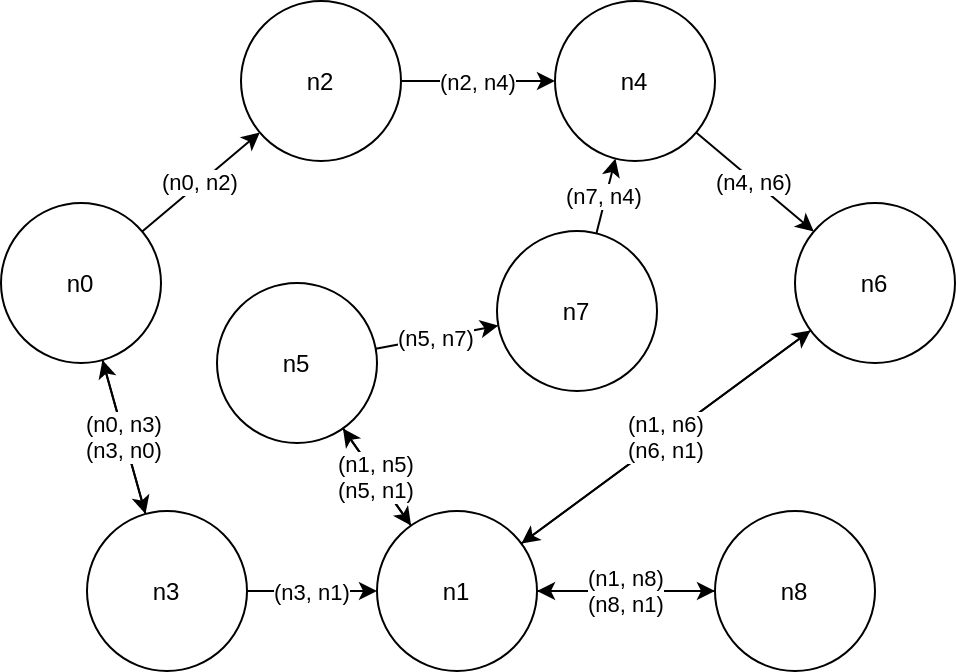
\includegraphics[width=.9\textwidth]{img/example_graph.png}
	\caption[Navegabilidad en los grafos dirigidos]{Un grafo dirigido es muy útil a la hora de representar problemas de navegabilidad, como por ejemplo en la búsqueda de caminos}
\end{figure}

Los grafos pueden tener restricciones, como por ejemplo de navegabilidad, pues decimos que un grafo es dirigido en el caso de que algún enlace solo pueda recorrerse en un único sentido.

Se dice que dos nodos son adyacentes si existe un enlace que una dichos nodos, si son vecinos. Esto nos permite definir los caminos, sucesiones ordenadas de nodos vecinos entre sí cuyo el punto de partida, el primer nodo, se denomina origen y su final, el último nodo, denota el objetivo.

\section{Topología}
La Topología \autocite[96]{volaya} es una disciplina matemática que estudia las características de objetos geométricos, como grafos, que no varían al aplicar una transformación, como mover un nodo de lugar. En el contexto GIS, la topología es generalmente definida \autocite{gfeTopo} como la relación espacial entre elementos vectoriales adyacentes o conectados entre sí. Es decir, en términos informales, una topología GIS es una estructura que nos detalla como están conectados los elementos. 

Estas relaciones, dicha estructura, permanecen constantes cuando se aplican ciertas deformaciones \autocite[310]{obehsu}, como un giro o una traslación, y nos permiten verificar la integridad de los datos. 

\begin{figure}[htbp]
	\centering
	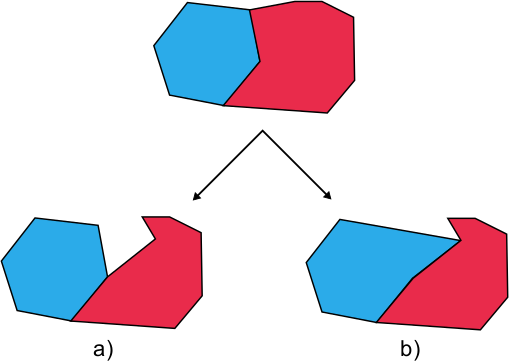
\includegraphics[width=.7\textwidth]{img/topo_modification.png}\\
	\autocite[97]{volaya}
	\caption[Topología geográfica y modificación]{Aplicación de una transformación a un punto sin (a) y con (b) información topológica}
\end{figure}

Un ejemplo real de esto es una red de autobuses, si en algún momento se moviese la ubicación de alguna parada, el conjunto de conexiones, o enlaces, seguiría siendo el mismo, exceptuando que dicha parada, o nodo, ha sido movida de lugar.

Los datos vectoriales no necesariamente deben contener información topológica  pero, generalmente, se puede obtener a través de un proceso de descomposición de primitivas, partiendo de todos los enlaces, y descomponiendo estos en subdivisiones entre nodos con un grado mayor que dos, o entre nodos origen y objetivo. Es decir, enlaces que contengan aquellos nodos que sean usados por algún otro enlace.

\section{Encaminamiento}
Una de las principales áreas de aplicación del Análisis de Redes es el encaminamiento, la búsqueda de caminos, generalmente basados en distancia (camino más corto) pero también en tiempo (camino más rápido). Indistintamente de cuál es la heurística principal, suelen darse un conjunto de condiciones adicionales, como la navegabilidad o pasaje por algún nodo intermedio.

\begin{figure}[htbp]
	\centering
	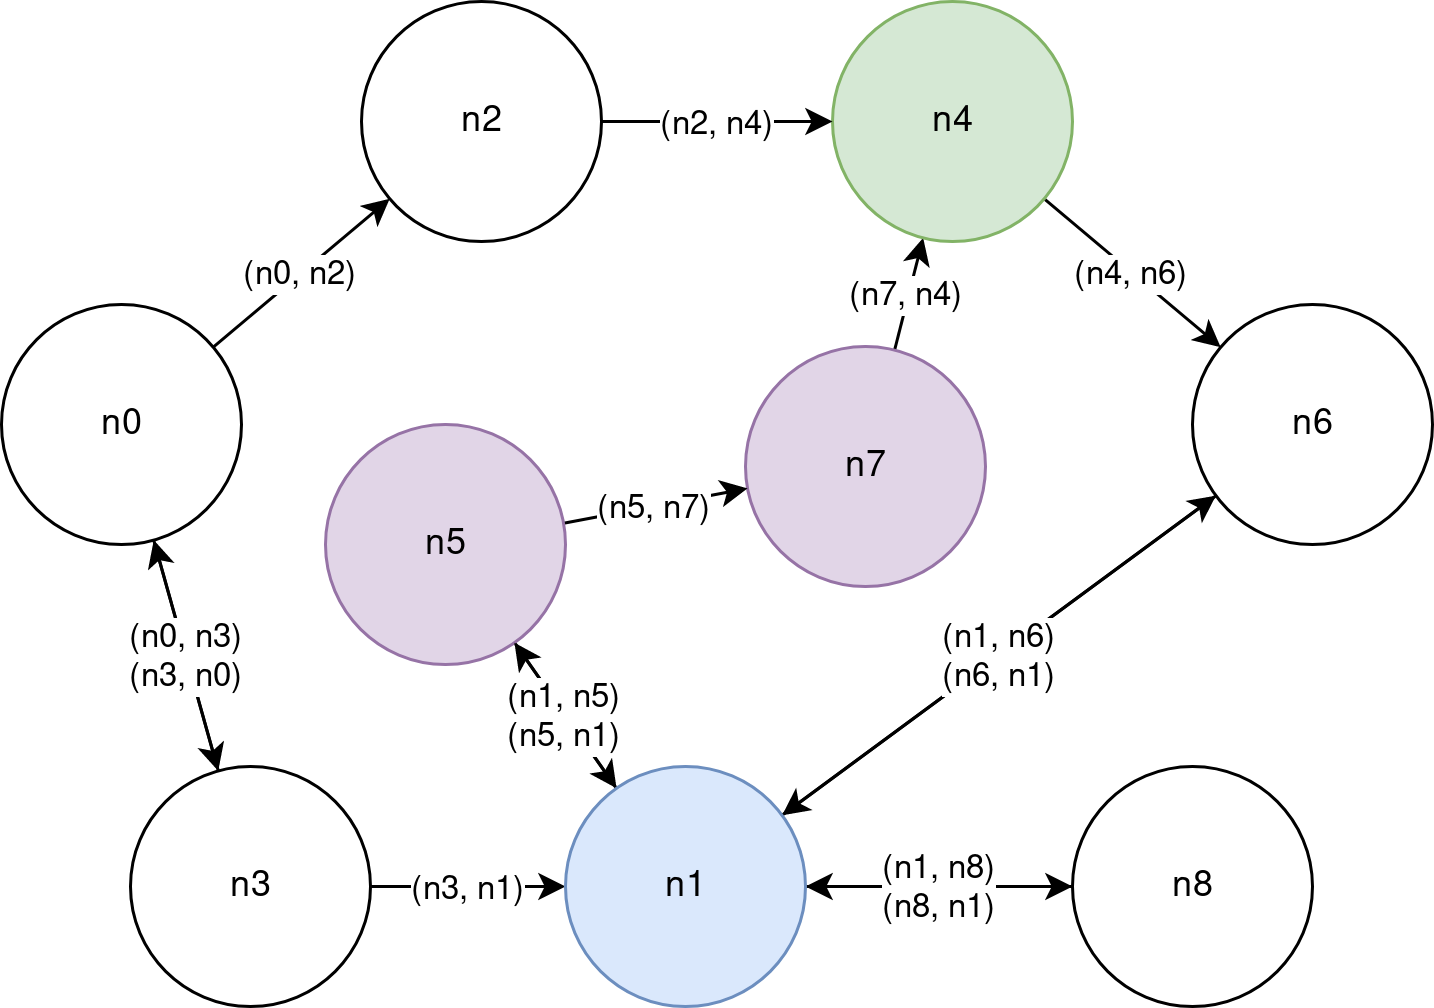
\includegraphics[width=.9\textwidth]{img/example_graph_path.png}
	\caption[Encaminamiento en un grafo dirigido]{Partiendo del origen $n1$ (en azul) y buscando llegar al destino $n4$ (en verde), se encuentra un camino (en lila) óptimo y, casualmente, único denotado como la secuencia de nodos $\left\lbrace n1, n5, n7, n4 \right\rbrace$ o la secuencia de enlaces $\left\lbrace (n1, n5), (n5, n7), (n7, n4) \right\rbrace$ a través de un algoritmo de búsqueda de caminos.}
\end{figure}

Esto tiene una sinergia tremenda con la información geográfica pues, como ya se ha comentado, podemos apreciar ciertos paralelismos entre grafos y datos geográficos. Aún así, este área no es algo sencillo, pero hay algoritmos muy conocidos, además de existir muchas herramientas que nos permiten trabajar con redes sobre las que aplicar técnicas de encaminamiento, comentadas a continuación.

\subsection{\textit{pgRouting}}
\textit{pgRouting} es una extensión de \textit{PostgreSQL} para el Análisis de Redes, concretamente en el ámbito de búsqueda de caminos \autocite[410-416]{obehsu}.

Como tal, al habilitar esta extensión en una base de datos, se nos permite el uso de las siguientes funciones, entre otras.

\begin{description}
	\item[\texttt{pgr\_CreateTopology}] Encargada de crear la topología de una entidad que contenga líneas vectoriales, descomponiendo cuando sea necesario.
	\item[\texttt{pgr\_Dijkstra}] Usada para buscar el camino más corto usando el algoritmo de \textit{Dijkstra}
\end{description}

Esto, con relativa sencillez, nos proporciona una herramienta muy eficaz para realizar búsqueda de caminos, pero está fuertemente ligada a la disposición de una base de datos \textit{PostgreSQL}, con \textit{PostGIS} y \textit{pgRouting}, limitando su despliegue en dispositivos con menos recursos.

\subsection{\textit{NetworkX}}
\textit{NetworkX} es un \textit{framework}\footnote{Conjunto de herramientas, marco de trabajo} de \textit{Python} para trabajar con grafos, y una excelente herramienta que nos permite aplicar encaminamiento en una red, al presentarse de manera agnóstica a ningún tipo de origen de datos, pero con un mayor coste en tiempo de preparación.
Incluso con esto dicho, también facilita mucho la integración con diferentes fuentes de datos, como por ejemplo con \textit{Shapefile}, \textit{CSV}, entre otros.

\begin{description}
	\item[\texttt{networkx.from\_pandas\_edgelist(df, *)}] Función para cargar un grafo a partir de un \textit{DataFrame} de  \textit{Pandas} o \textit{GeoPandas}.
	\item[\texttt{networkx.shortest\_path(G, b, e, *)}] Una función que toma un grafo y dos identificadores de nodos, realizando una búsqueda de camino de forma rápida.
\end{description}